\section{Hydraulics of sewer line}\label{se:hydraulics_of_sewer_line}
Methods to model hydraulics of gravity and pressurized sewer lines is explained respectively in the following. 
\fxnote{q beskrives sammen med store Q som flow, der er en fejl. ligning 3.27 mangler lidt forklaring. }

\subsection{Open channel}\label{subse:open_channel}
Modeling fluids is almost always done by considering it as a control volume. The reason is that it is rarely efficient, computational wise, or possible to consider the individual fluid particles.
Henceforth the control volume will be denoted by the letter $\Omega$ which will correspond to some amount of fluid in a length of sewer line.		

The open channel flow in gravity sewer lines can be described by the Saint-Venant equations which gives an expression for conservation of mass and momentum.
Some assumptions is made when deriving the Saint-Venant equations \cite{schutze2011modelling}:

\begin{table}[H]
\begin{enumerate}
\item The flow in the channel is one dimensional, and prismatic, and as such any curvature or change in width of the sewer line is considered negligible.
\item Fluid in the sewer line is considered incompressible and the pressure is assumed hydrostatic.
\item The only forces considered is friction, pressure and gravity.
\item The water height and velocity is uniform in the cross-section and only changes horizontally i.e. turbulence in the fluid is not considered.
\item The slope of the channel bed is small
% \item The flow in the sewer is one-dimensional, meaning that the water height and velocity is uniform in the cross-section and only changes horizontally.
% \item The curvature of the sewer line is sufficiently small such that it can be considered a straight line. 
% \item Vertical accelerations is neglected and the fluid is incompressible such that the pressure can be assumed hydrostatic.
% \item The slope and the variation in width of the sewer line is small.
% \item The effect of scour and accumulation of solids are assumed to be negligible. 
\end{enumerate}
\label{tab:saintbernard_assumptions}
\end{table}

\textbf{Continuity} equation for conservation of mass gives an expression for the amount of fluid flowing into the control volume and the flow out plus the fluid stored in it. 
In figure \ref{fig:firkant_kloak} a flow in a channel is shown. 
%The cross section is given as $A = h \cdot B$ which both is a function of position and time.

\begin{figure}[H]
\centering
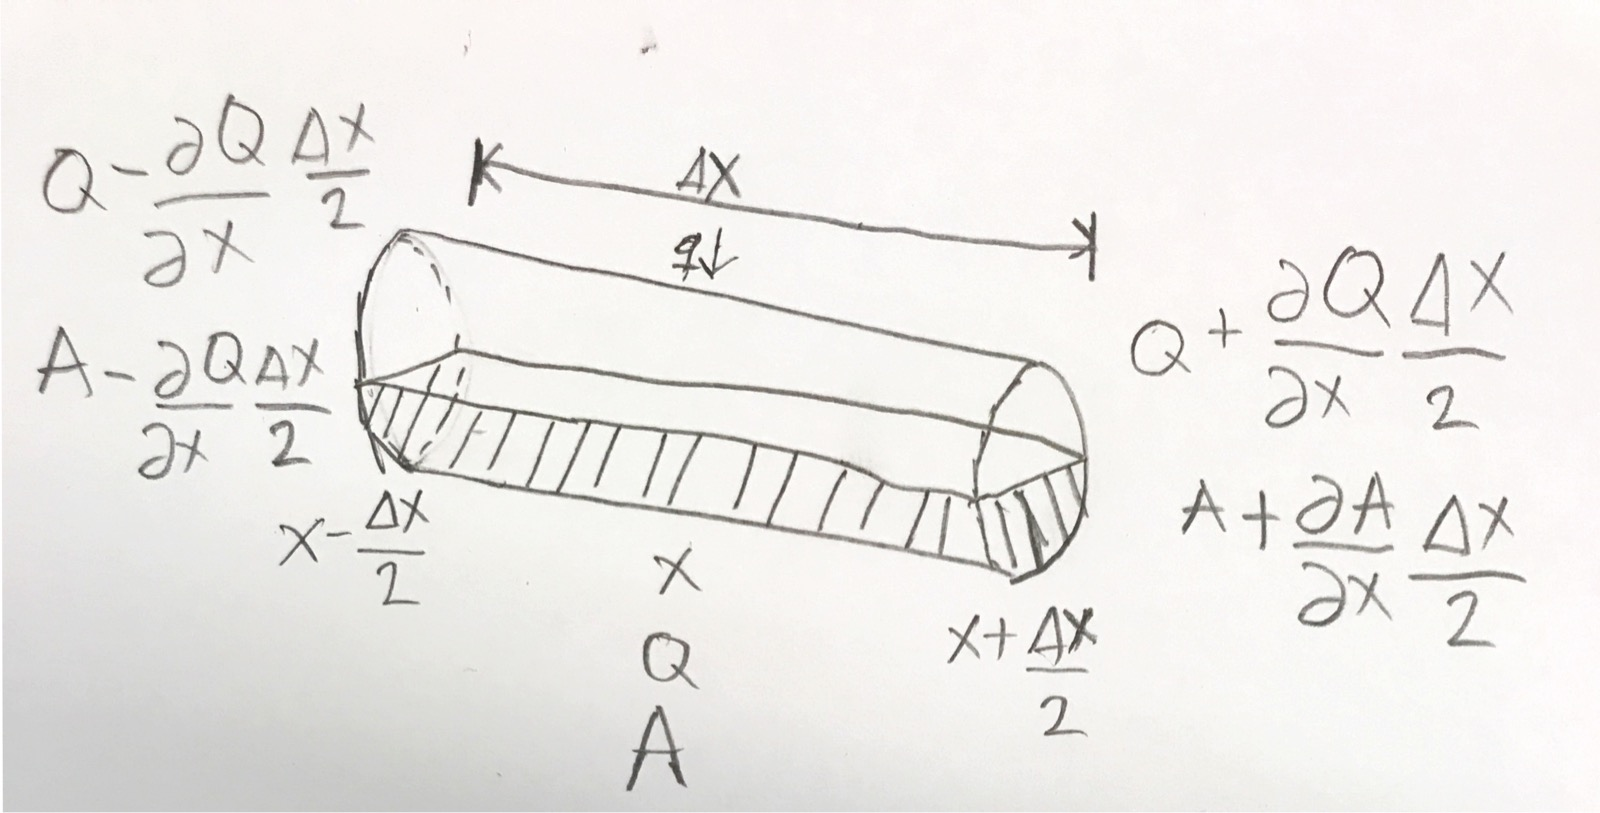
\includegraphics[width=0.8\textwidth]{report/modeling/pictures/continuity_open_channel.jpg}
\caption{Flow in a channel where Q is flow into the channel, q is lateral flow into the channel and A is the cross section area of the flow.}
\label{fig:firkant_kloak}
\end{figure}

The flows, Q, q and cross section area of the flow, A, shown in figure \ref{fig:firkant_kloak} is dependent on time and position, but in the following a simpler notation is used for an easier outline. 

The flow into the control volume where Q is the flow considered from the middle of the control volume is given as.

\begin{equation}
Q_{in} \cdot \Delta t =	\left(Q - \frac{\partial Q}{\partial x}\cdot \frac{\Delta x}{2}\right) \cdot \Delta t + q \cdot \Delta x \cdot \Delta t
\label{flowin_saintbernard}
\end{equation}

Where q is the lateral inflow across the entire channel [$\frac{m^2}{s}$] and Q is the flow in the channel [$\frac{m^3}{s}$]. Lateral inflow could for example come from adjoint sewer pipes or road drain.
The discharge flow of the channel is given as:

\begin{equation}
Q_{out} \cdot \Delta t =\left(Q + \frac{\partial Q}{ \partial x} \frac{\Delta x}{2} \right) \cdot \Delta t 
\label{flowout_saintbernard}
\end{equation}

Change in stored fluid in the channel is given as:

\begin{equation}\label{stored_saintbernard}
\frac{\partial}{\partial t} \left(\frac{\Delta x}{2} \cdot \left(A- \frac{\partial A}{\partial x} \frac{\Delta x}{2} +A + \frac{\partial A}{\partial x} \frac{\Delta x}{2}	\right) \right) \Delta t = \frac{\partial}{\partial t} \left(\frac{\Delta x}{2} \cdot \left( 2 A	\right) \right) \Delta t = \frac{\partial A}{\partial t} \cdot \Delta x	\Delta t
\end{equation}
%This can be simplified to:

% \begin{equation}
% 	\frac{\partial}{\partial t} \left(\frac{\Delta x}{2} \cdot \left( 2 A	\right) \right) \Delta t
% \end{equation}
% Which leads to:
% \begin{equation}\label{stored_saintbernardv2}
% 	\frac{\partial A}{\partial t} \cdot \Delta x	\cdot \Delta t
% \end{equation}

As the flow into the channel minus the flow out is equal to the change in stored fluid in the channel, then due to the assumption of incompressible fluid and uniformity the following can be written:  

\begin{equation}\label{eq:saintbernard_masse_simpel}
	Q_{in}\cdot \Delta t - Q_{out}\cdot \Delta t = \frac{\partial A}{\partial t} \cdot \Delta x	\cdot \Delta t
\end{equation}

Thereby inserting equations \ref{flowin_saintbernard} and \ref{flowout_saintbernard} in \ref{eq:saintbernard_masse_simpel} the following is obtained:

\begin{equation}
\begin{array}{l}
	\left(Q - \frac{\partial Q}{\partial x}\cdot \frac{\Delta x}{2}\right) \cdot \Delta t + q \cdot \Delta x \cdot \Delta t - \left(Q + \frac{\partial Q}{ \partial x} \frac{\Delta x}{2} \right) \cdot \Delta t  = \frac{\partial A}{\partial t}\cdot \Delta t 
	\cdot \Delta x \\ 
\Updownarrow \\
q \cdot \Delta x \cdot \Delta t  - \frac{\partial Q}{\partial x} \cdot \Delta x \cdot \Delta t  = \frac{\partial A}{\partial t} \cdot \Delta t 
	\cdot \Delta x 
\end{array}
\label{saintbernard_masse}
\end{equation}

Equation \ref{saintbernard_masse} can be reduced to the following by isolating and dividing with $\Delta x$ and $\Delta t$, on both sides, yielding the mass conservation part of the Saint-Venant equations.
\begin{equation}	
\frac{\partial A(x,t)}{\partial t} + \frac{\partial Q(x,t)}{\partial x}=q(x,t)
\label{saintbernard_mass_lateral}
\end{equation}

For channel flows without lateral input the mass conservation is given as:
\begin{equation}	
\boxed{\frac{\partial A(x,t)}{\partial t} + \frac{\partial Q(x,t)}{\partial x}=0}
\label{saintbernard_mass}
\end{equation}


\textbf{Momentum} of the control volume $\Omega$ shown in figure \ref{fig:momentum_picture} can be found by utilizing Newtons second law which says that force is equal to mass times acceleration.  
Basically this means that the momentum of the control volume can be found by integrating the sum of forces in the following differential equation:
\begin{equation}\label{eq:momentum_eq}
	\frac{d \mathcal{M}(t)}{dt} = \sum_{i}F_i(t)
\end{equation} 
Where $\mathcal{M}$(t) is the momentum, given as mass times a velocity vector, of the control volume at time t and $\text{F}_i$(t) is the various external forces affecting the control volume. It describes the movement of a mass that flows through a control volume, plus the sum of forces acting on the volume, which is equal to the velocity by which the movement of the mass is store in the control volume. In the following the forces acting upon the control volume will be elaborated. The forces are given by the hydrodynamic, hydrostatic, friction and gravity.

\begin{figure}[H]
\centering
\includegraphics[width=0.8\textwidth]{report/modeling/pictures/momentum_picture.png}
\caption{Illustration to derive the momentum equation on an open channel.}
\label{fig:momentum_picture}
\end{figure}


As already mentioned the derivate of the momentum is mass times the velocity which is equal to the force. Therefore the hydrodynamic force given by the fluid particles at each end of a infinite small slice of a control volume is given as:
\begin{equation}\label{eq:force_equal_vrhoQ}
	F= M \frac{dv}{dt} + \frac{dM}{dt} \cdot v 
\end{equation}
This is obtained by using the product rule for the derivate of the momentum. The forces is given as mass $[kg]$ times the acceleration $\left[\frac{m}{s^2}\right]$ plus the derivate of the mass times velocity $\left[\frac{m}{s}\right]$. As the acceleration is insignificant it is neglected due to the acceleration in a small slice is close to zero. The derivate of the mass is:
\begin{equation}\label{eq:mellem_regning_for_momentum}
	\frac{dM}{dt} = \rho \frac{dV}{t} = \rho\cdot Q
\end{equation}
Where the derivate of the mass is equal to the density times the derivate of the volume. The derivate of the volume V $\left[m^3\right]$ is equal to the mass flow Q $\left[\frac{m^3}{s}\right]$ and rho is the density $\left[\frac{kg}{m^3}\right]$. By inserting equation \ref{eq:mellem_regning_for_momentum} into equation \ref{eq:force_equal_vrhoQ} the force, given by the fluid particles at each end, can be written as:
\begin{equation}
	F = \rho\cdot Q\cdot v 
\end{equation}

The hydrodynamic force given by the in- and output of fluid particles in the control volume, with the assumption that the density of the fluid and the velocity of it in the cross section of the control volume is constant, is given as:

\begin{equation}
	F_{in}= \rho \cdot v \cdot Q - \frac{\partial}{\partial x}(\rho \cdot v \cdot Q) \cdot \frac{\Delta x}{2}
\end{equation}
\begin{equation}
	F_{out} = \rho \cdot v \cdot Q + \frac{\partial}{\partial x}(\rho \cdot v \cdot Q) \cdot \frac{\Delta x}{2}
\end{equation}

% \begin{equation}
% \left(\rho \cdot v \cdot Q - \frac{\partial}{\partial x}(\rho \cdot v \cdot Q) \cdot \frac{\Delta x}{2}\right)_{in} - \left(\rho \cdot v \cdot Q + \frac{\partial}{\partial x}(\rho \cdot v \cdot Q) \cdot \frac{\Delta x}{2} \right)_{out} 
% \end{equation}
Where subscript "\textit{in}" denote the force going in through the left side of the channel on figure \ref{fig:momentum_picture} and subscript "\textit{out}" is the force going out to the right side on figure \ref{fig:momentum_picture}.
The change of particle momentum in the control volume is given as $F_{in}- F_{out}$ and by replacing velocity with $Q/A$ the following is obtained:

\begin{equation}\label{mass_flow_speed}
\begin{array}{l}
\rho \cdot \frac{Q}{A} \cdot Q - \frac{\partial}{\partial x}\left(\rho \cdot \frac{Q}{A}  \cdot Q\right) \cdot \frac{\Delta x}{2} -\\ 
\left(\rho \cdot \frac{Q}{A}  \cdot Q + \frac{\partial}{\partial x}\left(\rho \cdot \frac{Q}{A}  \cdot Q\right) \cdot \frac{\Delta x}{2} \right)
= -  \rho\frac{\partial}{\partial x} \frac{Q^2}{A}\Delta x
\end{array}
\end{equation}

The remaining to be found is the forces imposed by gravity, friction and the hydrostatic.
The force applied by gravity is given as:
\begin{equation}
F_g = sin(\theta)\cdot g \cdot \rho \cdot \Delta x \cdot A
\label{gravity_force} 
\end{equation}

where the slope of the pipe bed $\text{S}_\text{b} = tan(\theta) \approx sin(\theta)$ for small values of $\theta$ resulting in:
\begin{equation}
F_g = S_b \cdot g \cdot \rho \cdot \Delta x \cdot A 
\end{equation}
The friction force can be set up as:
\begin{equation}
F_f = S_f \cdot g \cdot \rho \cdot \Delta x \cdot A 
\label{friction_force} 
\end{equation}
Where $S_f$ is a friction coefficient. This coefficient can be estimated by different formulas like Manning's or Darcy-Weishbach formula which is seen in equation \ref{Manning_formula} and \ref{darcy_weisbach_formula} respectively. 
\begin{equation}
	S_f = \frac{n^2 Q^2}{A^2R^{4/3}}= \frac{n^2 v^2}{R^{4/3}}
\label{Manning_formula}
\end{equation}
\begin{equation}
	S_f = \frac{f Q^2}{8gR A^2}= \frac{f v^2}{8gR}
\label{darcy_weisbach_formula}
\end{equation}

Where n is Manning's roughness factor, f is the Weisbach resistance coefficient and R is the hydraulic radius given as wetted area divided by the wetted perimeter \cite{stormwatercollectionsystems}.
The Weisbach resistance coefficient is found by the Colebrook-White formula seen in equation \ref{colebrook_white_formula}.
\begin{equation}
\frac{1}{\sqrt{f}} = -2\cdot log \left( \frac{k}{14.84 \cdot R}+ \frac{2.52}{4 Re \sqrt{f}} \right)
\label{colebrook_white_formula}
\end{equation}

Where f is the Darcy-Weisbach resistance coefficient, k is a pipe roughness coefficient and Re is the Reynolds number.

Last the hydrostatic forces on the x component of the control volume to be found is marked as $F_{P1}$ to $F_{P3}$ in figure \ref{fig:forces_on_CV}. 

\begin{figure}[H]
\centering
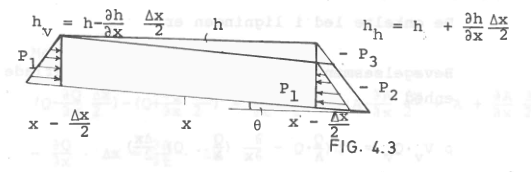
\includegraphics[width=0.75\textwidth]{report/modeling/pictures/palle_fig}
\caption{Forces acting on the control volume }
\label{fig:forces_on_CV}
\end{figure}\fxnote{Ny tegning og sikkert også caption}

The hydrostatic forces acting on the channel are found by taking a sectional view. Furthermore by assuming hydrostatic pressure across the channel, thus the pressure in a height z above the bottom of the channel is given as $g\rho(h-z)$, here h is the hight of the wastewater.  
The hydrostatic forces acting on the control volume to the left is given as:
\begin{equation}\label{eq:P1}
	F_{P1} = \int_{0}^{h_l} \rho \cdot g (h_l - z)\cdot b(z) dz
\end{equation}
Where $h_l$ is the water hight to the left of the channel, b(z) is the width of the channel given z. The hydrostatic force acting on the control volume to the right is given as:
\begin{equation}\label{eq:P2}
\begin{array}{l}
	-\int_{0}^{h_r} \rho \cdot g (h_r - z)\cdot b(z)dz = \\
	-\int_{0}^{h_l} \rho \cdot g (h_l - z)\cdot b(z)dz -\int_{0}^{h_l} \rho \cdot g (h_r- h_l)\cdot b(z)dz -\int_{h_l}^{h_r} \rho \cdot g (h_r - z)\cdot b(z)dz = \\
	-F_{P1} - F_{P2} - F_{P3}
\end{array}	
\end{equation}
The integral of $F_{P2}$ is: 
\begin{equation}
	F_{P2} = -\int_{0}^{h_l} \rho \cdot g (h_r - h_l)\cdot b(z)dz = -\rho g \frac{\partial h}{\partial x}\Delta x A_l
\end{equation}
Where $h_r$ is the water hight to the right of the channel. By assuming the width, b is constant the following can be approximated: 
\begin{equation}
	F_{P3}= -\int_{h_l}^{h_r} \rho \cdot g (h_r - z)\cdot b(z)dz \approx -\rho g b(h) \frac{1}{2}\left(\frac{\partial h}{\partial x}\Delta x\right)^2
\end{equation}	

Taking the sum of forces from equations \ref{eq:P1} and \ref{eq:P2}:
\begin{equation}
F_{P1} -F_{P1} -F_{P2} - F_{P3} =-\rho\cdot g \cdot \frac{\partial h}{\partial x} \cdot \Delta x \left(A_v + \frac{1}{2}b(h)\frac{\partial h}{\partial x} \Delta x \right) =-\rho\cdot g \cdot \frac{\partial h}{\partial x} \cdot \Delta x  \cdot A  
\label{pressure_force}
\end{equation}

By summing all the hydrostatic forces from equation \ref{mass_flow_speed}, \ref{gravity_force}, \ref{friction_force} and \ref{pressure_force} they can be inserted into equation \ref{eq:momentum_eq}:

\begin{equation}
\frac{d \mathcal{M}(t)}{dt}	=- \frac{\partial}{\partial x} \rho \frac{Q^2}{A}\Delta x
-S_b \cdot g \cdot \rho \cdot \Delta x \cdot A -S_f \cdot g \cdot \rho \cdot \Delta x \cdot A  -\rho\cdot g \cdot \frac{\partial h}{\partial x} \cdot \Delta x \cdot A
\label{eq:sum_of_forces}
\end{equation}

Lastly the time derivative expression of the momentum, which is given by mass times velocity, are:

\begin{equation}\label{eq:leftside_momentum}
	\frac{\partial}{\partial t} \left(\rho \frac{Q}{A}A\Delta x\right)
\end{equation}
Where mass is given by $\rho \cdot A \cdot \Delta x$ and velocity by $Q / A$.

Thereby all the sum of forces from equation \ref{eq:sum_of_forces} can be set equal to  \ref{eq:leftside_momentum}.% Adding equation \ref{mass_flow_speed}, \ref{gravity_force}, \ref{friction_force} and \ref{pressure_force} an expression is given for the velocity of storing fluid in the control volume which is equal to:
% \begin{equation}
% \frac{\partial}{\partial t}(\rho\cdot v \cdot A\cdot \Delta x) = \frac{\partial}{\partial t} (\rho \frac{Q}{A}A\cdot \Delta x)
% \end{equation}

\begin{equation}
\begin{array}{l}
%\rho \cdot \frac{Q}{A} \cdot Q - \frac{\partial}{\partial x}(\rho \cdot \frac{Q}{A}  \cdot Q) \cdot \frac{\Delta x}{2} - \left(\rho \cdot \frac{Q}{A}  \cdot Q - \frac{\partial}{\partial x}(\rho \cdot \frac{Q}{A}  \cdot Q) \cdot \frac{\Delta x}{2} \right)\\
% \frac{\partial}{\partial t} (\rho \frac{Q}{A}A\cdot \Delta x) =- \frac{\partial}{\partial x} \rho \frac{Q^2}{A}\Delta x
% -S_b \cdot g \cdot \rho \cdot \Delta x \cdot A -S_f \cdot g \cdot \rho \cdot \Delta x \cdot A  \\-\rho\cdot g \cdot \frac{\partial h}{\partial x} \cdot \Delta x \cdot A 
\frac{\partial}{\partial t} (\rho \frac{Q}{A}A\cdot \Delta x) = - \frac{\partial}{\partial x} \rho \frac{Q^2}{A}\Delta x -S_b \cdot g \cdot \rho \cdot \Delta x \cdot A -S_f \cdot g \cdot \rho \cdot \Delta x \cdot A \\ 
-\rho\cdot g \cdot \frac{\partial h}{\partial x} \cdot \Delta x \cdot A 

\end{array}
\end{equation}
\\
Dividing with $\Delta x \rho g A$ and isolating then the following definition of the equation is obtained:
\\
\begin{equation}
\boxed{\frac{1}{gA} \frac{\partial Q}{\partial t} +\frac{1}{gA}\frac{\partial}{\partial x} \left( \frac{Q^2}{A} \right) + \frac{\partial h}{\partial x} + S_f - S_b = 0}
\label{saintbernard_momentum}
\end{equation}
\\

Some or all of the terms in equation \ref{saintbernard_momentum} can be utilized when simulating free channel flow. An overview of the limitations when excluding parts of the momentum equation is given in table \ref{momentum_approximations}.

\begin{table}[H]
\centering

\begin{tabular}{|l|l|l|l|l|} \hline
%\rowcolor[HTML]{9B9B9B}
\multirow{2}{*} {Approximation} &   Kinematic & \multirow{2}{*} {Noninertia (2)}  & Quasi-steady  & Dynamic \\
			 					&  	wave (1)   &  			 					 & dynamic wave (3) 	& wave (4)  \\ \hline

 \multirow{2}{*} {momentum equation} 		&\multirow{2}{*} {$S_b = S_f$}  & \multirow{2}{*} {$\frac{\partial h}{\partial x}= S_b- S_f$ } & $\frac{1}{gA}\frac{\partial}{\partial x} \left( \frac{Q^2}{A} \right) + \frac{\partial h}{\partial x}$ & \multirow{2}{*} {equation \ref{saintbernard_momentum}} \\
%\rowcolor[HTML]{9B9B9B} 
&  &  & = $S_b - S_f$  &  \\ \hline

Boundary conditions &\multirow{2}{*} 1 &\multirow{2}{*} 2  &\multirow{2}{*} 2 &\multirow{2}{*} 2 \\ 
required&  &  &  &  \\ \hline

 Account for 			& \multirow{4}{*} {No} &\multirow{4}{*} {Yes}  & \multirow{4}{*} {Yes}  & \multirow{4}{*} {Yes}  \\
 downstream backwater	&  &  &  &  \\
 effect and flow 		&  &  &  &  \\
 reversal 				&  &  &  &  \\ \hline

Damping of & \multirow{2}{*} {No}  & \multirow{2}{*} {Yes} & \multirow{2}{*} {Yes}  & \multirow{2}{*} {Yes} \\ 
flood peak &  &  &  &  \\ \hline

Account for & \multirow{2}{*} {No}  & \multirow{2}{*} {No} & only convective & \multirow{2}{*} {Yes} \\
flow acceleration &  &  & acceleration  &  \\ \hline
\end{tabular}
\caption{Limitations when excluding, 1.(inertia and pressure terms), 2.(inertia terms), 3.(pressure term relating to local acceleration) and 4.(none), from the momentum equation \cite{stormwatercollectionsystems}. }
\label{momentum_approximations}
\end{table} 

The kinematic wave is the simplest approximation and ignores the terms representing changes in inertia and pressure by assuming that the slope of the water surface is identical to that of the channel bed. 
This means that the flow is uniform across an interval $\Delta x$ at a given $\Delta t$ and mechanisms for flood wave peak attenuation is disregarded. Due to the simplicity of the kinematic wave approximation, attenuation which occurs in a real free flowing channel should not be present. Numerical damping can be induced because of the nature of discretization, but mistakenly corrections has been attempted to mitigate the attenuation by choosing smaller step sizes of $\Delta x$ and $\Delta t$, where instead attempts should be made, to fit the sizes, to imitate the natural attenuation of the free flowing channel.     
Furthermore only one boundary condition is required, which is specified upstream, meaning that any backwater effects such as storing is neglected. This also means that simulation can be done without knowing the lower end boundary of the channel flow. Because of its simplicity the momentum equation in the form of the kinematic wave approximation has been used and researched extensively\cite{stormwatercollectionsystems}.  


%\begin{figure}[H]
%\centering
%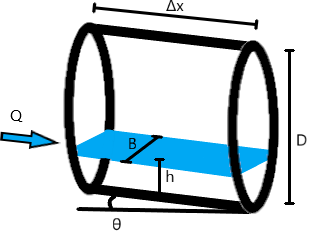
\includegraphics[width=0.45\textwidth]{report/modeling/pictures/kloakroer.png}
%\caption{Sewer pipe \fxnote{Ny tegning indsæt omega i control volumet}}
%\label{fig:kloakroer}
%\end{figure}


%\begin{equation}
%\frac{1}{gA} \frac{\partial Q}{\partial t} +\frac{1}{gA}\frac{\partial}{\partial x} \left( \frac{Q^2}{A} \right) + \frac{\partial h}{\partial x} + S_f - S_b = 0
%\label{saintbernard_momentum}
%\end{equation}

%\begin{equation}
%\frac{1}{gA} \frac{\partial Q}{\partial t} +\frac{1}{gA}\frac{\partial}{\partial x} \left( \frac{Q^2}{A} \right) + cos (\theta) \frac{\partial h}{\partial x} + S_f - S_b = 0
%\end{equation}



%\begin{equation}
%	\frac{\partial Q(x,t)}{\partial t} + \frac{\partial}{\partial x} \frac{ Q^2(x,t)}{A(x,t)}+ g \cdot A(x,t) (\frac{\partial h(x,t)}{\partial x} +S_f(x,t)-S_b(x)) = 0
%\label{saintbernard_momentum}
%\end{equation}




